\newpage
\section{Servoberäkningar}
\label{servoberakningar}

Servoberäkningarna tillkommer som underlag för objektidentifiering i ~\ref{objektidentifiering}. Nedan behandlas samtliga beräkningar för de fyra servomotorer som styr tummen och pekfingret.


\subsection{Beräkningar för servomotor 1}

Servomotor 1 är med hjälp av ett stag kopplat till tummens första led och styr därmed dess rörelsevinkel $\alpha$, se figur \ref{fig:servo2}. 

\begin{figure}[H]
\includegraphics[width=0.5\textwidth]{img/servo/servo_berakning11}
\caption{Rörelse i tummens första led till följd av rörelse i servomotor 1}
\label{fig:servo1}
\end{figure}

Bild \ref{fig:servo2} nedan visar hur servomotorn är kopplat via ett stag till tummens första led. Servot har sin roterande axel i punkt $P_{0}$ vilken sedan är förskjutet till punkt $P_{1}$ med hjälp av ett servokors med radie $R_{1}$. Servokorset drar i sin tur i ett stag med längden c som påverkar tummens första led. Leden kan rotera kring punkt $P_{3}$ vilket ger upphov till en vinkel $\alpha$.


\begin{figure}[H]

\includegraphics[width=0.55\textwidth]{img/servo/servo1}
\caption{Nödvändiga beteckningar för beräkningar till servomotor 1}
\label{fig:servo2}
\end{figure}

\[
\begin{cases}
r_{1}=\unit[16]{mm} \\
r_{2}=\unit[12]{mm}\\
a=\unit[4]{mm}\\
b=\unit[55]{mm}\\
c=\unit[58]{mm} \\
\end{cases}
\]

\begin{table}[H]
    \begin{tabular}{|c|l|l|}
        \hline
        Punkt  & X-Koordinat & Y-Koordinat                       \\ \hline
  $P_{0}$      & 0   & 0                                   \\ \hline
  $P_{1}$      & $r_{1}\cos(\varphi)$ & $r_{1}\sin(\varphi)$              \\ \hline
  $P_{2}$      & $P_{3x}-r_{2}\sin(\alpha)$  & $P_{3y}+r_{2}\cos(\alpha)$                  \\ \hline
  $P_{3}$      & $b$ & $-a$ \\ \hline
    \end{tabular}
\end{table}


Avståndet mellan punkterna $P_{2}$ och $P_{1}$ är  alltid c vilket är längden på staget som sammankopplar de båda punkterna. Detta utnyttjas för att upprätta ett itterations villkor. Ett gissat värde på alfa ($\alpha_{guess}$) ger koordinaterna för punkt $P_{2}$ vilket i sin tur ger ett avstånd mha avståndsformeln, se itterationsschemat \ref{itteration} nedan. På så sätt kan ett specifikt $\alpha$ fås för varje servovinkel $\varphi$.



\begin{flushleft}
\label{itteration}
 (1)   $\varphi,\alpha_{guess}$ $\rightarrow$ \\
  (2)  $P_{1}=[r_{1}\cos(\varphi),r_{1}\sin(\varphi)]$ $\rightarrow$
  \\(3) \thinspace $P_{2}=[P_{3x}-r_{2}\sin(\alpha_{guess}),P_{3y}+r_{2}\cos(\alpha_{guess})]$ $\rightarrow$ \\
  (4)\ $c_{g}=\sqrt[]{(P_{1x}-P_{2x})^2+(P_{1y}-P_{2y})^2}$ $\rightarrow$\\(5) Kolla om: $|c-c_{g}|>tol$ \\ (6) Om (5) stämmer $\rightarrow$ $\alpha_{guess}=\alpha_{guess}+value$ \ , \ börja om från punkt (3) \\ annars $\rightarrow$ det approximativa $\alpha$-värdet har hittats
\end{flushleft}

Med hjälp av matlab så har ovanstående itterationsshema genererat ett $\alpha$-värde för varje servoläge ($\varphi$). Detta utnyttjades sedan med minsta kvadratmetoden för att ta fram ekvation \eqref{eq:servo1} utifrån dessa värden.

\begin{equation}
\label{eq:servo1}
\alpha= A\varphi^4+B\varphi^3+C\varphi^2+D\varphi+E
\end{equation}

\begin{table}[H]
    \begin{tabular}{|c|l|}
        \hline
        A      & 0.000005730076566  \\ \hline
        B      & -0.000776743538556  \\ \hline
        C      & 0.050190358704910    \\ \hline
        D      & -0.929487032616965    \\ \hline
        E      & 5.269186999542453      \\ \hline
    \end{tabular}
\end{table}


\begin{figure}[H]
\label{servo3}
\includegraphics[width=0.7\textwidth]{img/servo/alfa_servo_0}
\caption{$\alpha$-vinkeln som en funktion av servovinkeln $\varphi$}
\end{figure}

Genom att anpassa en ekvation till kurvan undviks itterationsprocessen vid styrning av handen vilket underlättar för processorn. Med hjälp av ekvation \eqref{eq:servo2} kan koordinaterna för ytterpunkterna på tummens första led beräknas. Tummens origo är placerat i dess första roterande punkt, punkt $P_{3}$ i figur  \ref{fig:servo2}. 

\begin{equation}
\label{eq:servo2}
P1_{tumme}=[L_{1}\sin(\alpha),L_{1}\cos(\alpha)]
\end{equation}


\begin{center}
$L_{1}=39mm$
\end{center}

\newpage

\subsection{Beräkningar för servomotor 2}
\label{servo2}

Servomotor 2 styr tummens andra led genom att applicera en kraft på en sena kopplat till ledens mittpunkt, punkt $P_{2}$ i figur \ref{fig:servo5}. Fingrets rörelse illustreras i figur  \ref{fig:servo4}

\begin{figure}[H]
\includegraphics[width=0.5\textwidth]{img/servo/servo_berakning2}
\caption{Rörelse i tummens andra led till följd av rörelse i servo 2}
\label{fig:servo4}
\end{figure}


\begin{minipage}[t]{0.5\textwidth}
\begin{figure}[H]
\includegraphics[width=0.8\textwidth]{img/servo/servo_berakning22}
\caption{Definition av längder}
\label{fig:servo5}
\end{figure}
\end{minipage}
\begin{minipage}[t]{0.5\textwidth}
\begin{figure}[H]
\includegraphics[width=1\textwidth]{img/servo/servo_berakning23}
\caption{Definition av vinklar}
\label{fig:servo6}
\end{figure}
\end{minipage}

\[
\begin{cases}
a=\unit[24]{mm} \\
b=\unit[39]{mm}\\
\theta=\frac{\pi}{4}\\
\end{cases}
\]

Servomotorn minskar avståndet c linjärt genom att linda senan runt servohjulet. Därav blir avståndsminskningen (s) proportionellt med servoläget($\varphi$) och servohjulets radie ($r_{s}$)enligt ekvation \eqref{eq:servo3}

\begin{equation}
\label{eq:servo3}
s=r_{s}\varphi
\end{equation}

Senans ursprungslängd betecknas $c_{0}$ och fås när servomotorn står i sitt minsta läge ($\varphi_{0}$). Vid detta servoläge gäller att:

\begin{center}
$\beta=0$ $\rightarrow$ $\gamma_0=\pi-\theta=\frac{3\pi}{4}$
\end{center}

Med hjälp av cosinus-satsen fås sedan $c_0$ genom ekvation \eqref{eq:servo4}

\begin{equation}
\label{eq:servo4}
c_0=\sqrt[]{a^2+b^2-2ab\cos(\gamma_0)}=61.8mm
\end{equation}


När $c_0$ är bestämmd kan $\beta$ fås för varje servoläge genom ekvationer \eqref{eq:servo5}-\eqref{eq:servo6}


\begin{equation}
\label{eq:servo5}
\gamma=\arccos(\frac{a^2+b^2-(c_0-s)^2}{2ab})
\end{equation}


\begin{equation}
\label{eq:servo6}
\beta=\pi-\theta-\gamma
\end{equation}

\begin{figure}[H]
\label{fig:servo7}
\includegraphics[width=0.7\textwidth]{img/servo/beta_servo_0}
\caption{$\beta$-vinkel som funktion av servovinkel ($\varphi$)}
\end{figure}

\begin{equation}
\label{eq:servo10}
\beta= A\varphi^4+B\varphi^3+C\varphi^2+D\varphi+E
\end{equation}

\begin{table}[H]
    \begin{tabular}{|c|l|}
        \hline
        A      & -0.000001953004447 \\ \hline
        B      & 0.000371410356959   \\ \hline
        C      & -0.028504560185942   \\ \hline
        D      & 1.756616442878862     \\ \hline
        E      &  0.451424425453001     \\ \hline
    \end{tabular}
\end{table}



\begin{figure}[H]
\label{fig:servo75}
\includegraphics[width=0.7\textwidth]{img/servo/servo_berakning24}
\caption{Definition av tummens punkter}
\end{figure}


När $\beta$ är bestämd kan övrig punkter bestämmas med hjälp av ekvationer \eqref{eq:servo7}-\eqref{eq:servo9}

\begin{equation}
\label{eq:servo7}
\mu=\alpha+\beta-\frac{\pi}{4}
\end{equation}

\begin{equation}
\label{eq:servo8}
P_2=[P_{1x}+L_2\cos(\frac{\pi}{2}-\alpha-beta),P_{1y}+L_2\sin(\frac{\pi}{2}-\alpha-beta)]
\end{equation}

\begin{equation}
\label{eq:servo9}
P_3=[P_{2x}+L_3\cos(\mu),P_{1y}-L_3\sin(\mu)]
\end{equation}

\begin{table}[H]
    \begin{tabular}{|c|l|}
        \hline
        $L_2$      & 13[mm] \\ \hline
        $L_3$      & 39[mm]  \\ \hline

    \end{tabular}
\end{table}

\newpage
\subsection{Beräknar för servomotor 3}

Servomotor 3 är, precis som servomotor 1 kopplat med ett stag och kontrollerar därmed fingrets $\alpha$-vinkel vilket illustreras i figur \ref{fig:servo8}

\begin{figure}[H]
\includegraphics[width=0.5\textwidth]{img/servo/servo_berakning3}
\caption{Rörelse i pekfingrets första led till följd av rörelse i servomotor 3}
\label{fig:servo8}
\end{figure}



\begin{figure}[H]

        \begin{subfigure}[b]{0.5\textwidth}
                \centering
                \includegraphics[width=\textwidth]{img/servo/servo_berakning31}
                \caption{Stagkonstruktion i sitt ursprungsläge}
                \label{fig:servo9}
        \end{subfigure}%
        ~ %add desired spacing between images, e. g. ~, \quad, \qquad etc.
          %(or a blank line to force the subfigure onto a new line)
        \begin{subfigure}[b]{0.5\textwidth}

                \includegraphics[width=\textwidth]{img/servo/servo_berakning32}
                \caption{Stagkonstruktion efter servorörelse}
                \label{fig:servo10}
        \end{subfigure}
\end{figure}

Servomotor 3 påverkar så som servomotor 1, ledens $\alpha$-vinkel med hjälp av ett stag. Konstruktionen har två fasta punkter, $P_0$ samt $P_3$ med koordinaterna som listas nedan. Servomotorn har sin axel i punkt $P_0$ som därifrån är kopplat med hjälp av ett servokors till fingerstaget. Genom att applicera avståndsformeln mellan punkt $P_1$ och $P_2$ kan ett $\alpha$ ittereras fram med villkoret att: $\sqrt[]{(P_{1x}-P_{2x})^2+(P_{1y}-P_{2y})^2}=c$


\begin{table}[H]
    \begin{tabular}{|c|l|}
        \hline
        $a$      & $\unit[8]{mm}$ \\ \hline
        $b$      & $\unit[122]{mm}$  \\ \hline
        $r_1$    & $\unit[16]{mm}$  \\ \hline
        $r_2$    & $\unit[26]{mm}$  \\ \hline
        $\varphi_0$ & $\frac{\pi}{12}$  \\ \hline
    \end{tabular}
\end{table}

\begin{equation}
\begin{split}
P_0 &= [0,0] \\
P_3 & =[-b,a] \\
c &= \sqrt[]{(b+r_1\cos(\varphi_0))^2+r_2^2}=132[mm]\\
P_1 &= [r_1\cos(\varphi),r_1\cos(\varphi)]\\
P_2 &= [-b-r_2sin(\alpha),a+r_2\cos(\alpha)]
\end{split}
\end{equation}

Resultatet av iterationen visas i figur \ref{fig:servo11} och är approximerat i ekvation \eqref{eq:servo11} med hjälp av minsta kvadratmetoden.

\begin{figure}[H]
\caption{$\alpha$-vinkel som funktion av servoläge}
\includegraphics[width=0.7\textwidth]{img/servo/alfa_servo_1}
\label{fig:servo11}
\end{figure}

\begin{equation}
\label{eq:servo11}
\alpha= A\varphi^4+B\varphi^3+C\varphi^2+D\varphi+E
\end{equation}

\begin{table}[H]
    \begin{tabular}{|c|l|}
        \hline
        A      & 0.000001356501825  \\ \hline
        B      & -0.000304772265970  \\ \hline
        C      & 0.027512021238403    \\ \hline
        D      & -0.540303738165201    \\ \hline
        E      & 3.396572953164549      \\ \hline
    \end{tabular}
\end{table}

\newpage

\subsection{Beräknar för servomotor 4}
Beräkningar för pekfingrets $\beta$-vinkeln följer exakt samma struktur som beräkningar för tummens $\beta$-vinkeln som går att hitta i avsnitt \ref{servo2}. Undantaget är de olika parametervärden. Nedan listas det parametervärden som är essentiella i följande beräkning.

\begin{figure}[H]
\label{fig:servo12}
\includegraphics[width=0.5\textwidth]{img/servo/servo_berakning4}
\caption{Rörelse i pekfingrets andra led till följd av rörelse i servomotor 4}
\end{figure}

\[
\begin{cases}
a=\unit[26]{mm} \\
b=\unit[52]{mm}\\
r_s=12[mm]\\
c_o=77[mm]\\
\end{cases}
\]

\begin{figure}[H]
\label{fig:servo13}
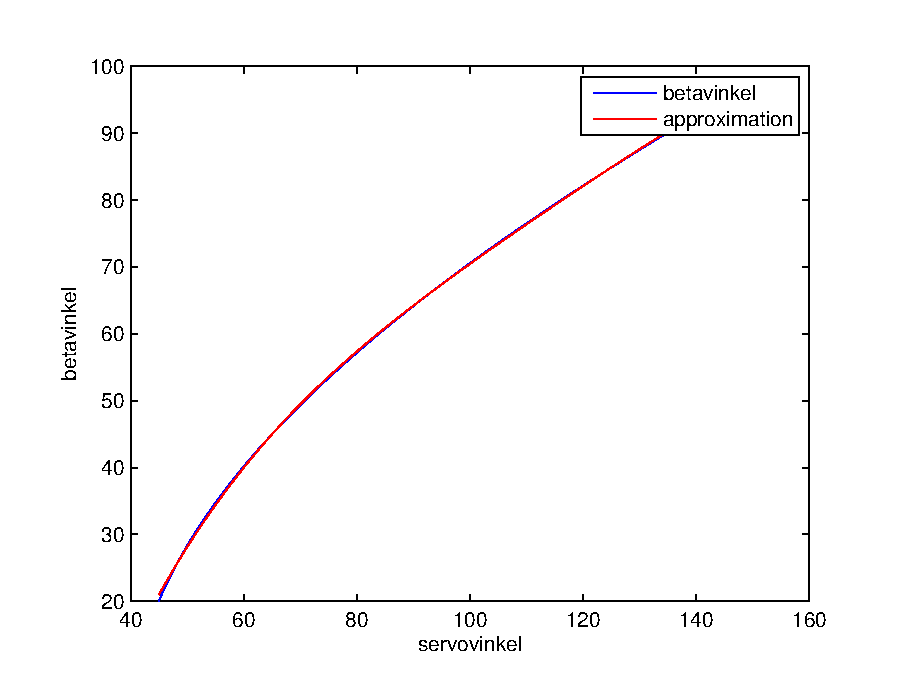
\includegraphics[width=0.7\textwidth]{img/servo/beta_servo_1}
\caption{$\beta$-vinkel som funktion av servoläge}
\end{figure}

\begin{equation}
\label{eq:servo12}
\beta= A\varphi^4+B\varphi^3+C\varphi^2+D\varphi+E
\end{equation}

\begin{table}[H]
    \begin{tabular}{|c|l|}
        \hline
        A      & -0.0000006147645\\ \hline
        B      & 0.0002814025560  \\ \hline
        C      & -0.0490932574478  \\ \hline
        D      & 4.4394812352849    \\ \hline
        E      & -102.5084186285169  \\ \hline
    \end{tabular}
\end{table}

Pekfingrets rörelse som funktion av $\alpha$ och $\beta$ fås med hjälp av det rymdekvationer som är specade i avsnitt \ref{rymdekv}. 
